%%% LaTeX Template: Two column article
%%%
%%% Source: http://www.howtotex.com/
%%% Feel free to distribute this template, but please keep to referal to http://www.howtotex.com/ here.
%%% Date: February 2011

%%% Preamble
\documentclass[	DIV=calc,%
							paper=a4,%
							fontsize=12pt,%
							onecolumn]{scrartcl}	 					% KOMA-article class

\usepackage{lipsum}													% Package to create dummy text
\usepackage[brazil]{babel}										% English language/hyphenation
\usepackage[protrusion=true,expansion=true]{microtype}				% Better typography
\usepackage{amsmath,amsfonts,amsthm}					% Math packages
\usepackage[pdftex]{graphicx}									% Enable pdflatex
\usepackage[svgnames]{xcolor}									% Enabling colors by their 'svgnames'
\usepackage[hang, small,labelfont=bf,up,textfont=it,up]{caption}	% Custom captions under/above floats
\usepackage{epstopdf}												% Converts .eps to .pdf
\usepackage{subfig}													% Subfigures
\usepackage{booktabs}												% Nicer tables
\usepackage{fix-cm}													% Custom fontsizes
\usepackage[utf8]{inputenc}
\usepackage[top=2.5cm, bottom=2.5cm, left=2.5cm, right=2.5cm]{geometry}
\usepackage[ddmmyyyy]{datetime}
\addto\captionsenglish{%
	\renewcommand\tablename{Tabela}
	\renewcommand\figurename{Figura}
} 
 

 
%%% Custom sectioning (sectsty package)
\usepackage{sectsty}													% Custom sectioning (see below)
\allsectionsfont{%															% Change font of al section commands
	\usefont{OT1}{phv}{b}{n}%										% bch-b-n: CharterBT-Bold font
	}

\sectionfont{%																% Change font of \section command
	\usefont{OT1}{phv}{b}{n}%										% bch-b-n: CharterBT-Bold font
	}



%%% Headers and footers
\usepackage{fancyhdr}												% Needed to define custom headers/footers
	\pagestyle{fancy}														% Enabling the custom headers/footers
\usepackage{lastpage}	

% Header (empty)
\lhead{}
\chead{}
\rhead{}
% Footer (you may change this to your own needs)

%% ====================================
%% ====================================
%% mude o rodape  do projeto
%% ====================================
%% ====================================

\lfoot{\footnotesize \texttt{Cabeamento estruturado} \textbullet ~ Projeto de Redes da empresa JSG}


\cfoot{}
\rfoot{\footnotesize página \thepage\ de \pageref{LastPage}}	% "Page 1 of 2"
\renewcommand{\headrulewidth}{0.0pt}
\renewcommand{\footrulewidth}{0.4pt}



%%% Creating an initial of the very first character of the content
\usepackage{lettrine}
\newcommand{\initial}[1]{%
     \lettrine[lines=3,lhang=0.3,nindent=0em]{
     				\color{DarkGoldenrod}
     				{\textsf{#1}}}{}}



%%% Title, author and date metadata
\usepackage{titling}															% For custom titles

\newcommand{\HorRule}{\color{DarkGoldenrod}%			% Creating a horizontal rule
									  	\rule{\linewidth}{1pt}%
										}

\pretitle{\vspace{-30pt} \begin{flushleft} \HorRule 
				\fontsize{50}{50} \usefont{OT1}{phv}{b}{n} \color{DarkRed} \selectfont 
				}

%% ====================================
%% ====================================
%% mude o titulo  do projeto
%% ====================================
%% ====================================

\title{ Projeto de Redes da empresa JSG}					% Title of your article goes here

%% ====================================



\posttitle{\par\end{flushleft}\vskip 0.5em}

\preauthor{\begin{flushleft}
					\large \lineskip 0.5em \usefont{OT1}{phv}{b}{sl} \color{DarkRed}}
\author{Heltton Mendonça Mendes Maciel }  	% Author name goes here


\postauthor{\footnotesize \usefont{OT1}{phv}{m}{sl} \color{Black} 
					\\Transportadora JSG - Departamento de Tecnologia da informação								% Institution of author
					\par\end{flushleft}\HorRule}

\date{}																				% No date




%%% Begin document
\begin{document}
\maketitle
\thispagestyle{fancy} 	
\thispagestyle{empty}		% Enabling the custom headers/footers for the first page 
% The first character should be within \initial{}




%% ====================================
%% ====================================
%% mude o resumo  do projeto
%% ====================================
%% ====================================
\initial{E}\textbf{este documento detalha o projeto de  implantação de uma nova estrutura de redes da transportadora JSG, empresa que possui duas unidades na cidade de Curitiba. 
Esse projeto prevê a interligação logica entre as unidades, a construção da estrutura fisica necessária, equipamentos a ser utilizado, definição das tecnologias, marcas, tipo de cabeamento e documentação da rede. }

%% ====================================
\begin{figure}
	\centering
	
\includegraphics{utfpr}
\end{figure}

\vspace{3cm}
\centerline{\textit{\textbf{\today}}}

\clearpage
    \renewcommand*\listfigurename{Lista de figuras}
\listoffigures

\renewcommand*\listtablename{Lista de tabelas}
\listoftables




\clearpage
\renewcommand{\contentsname}{Sumário}
\tableofcontents
\clearpage

%% ====================================
%% ====================================
%% Inicio do texto
%% ====================================
%% ====================================
\section{Introdução}
	A transportadora JSG é uma empresa de grande porte com duas unidades na cidade de Curitiba, é responsável pelo transporte dos caminhões que saem da fábrica da Volvo, tratores e colheitadeiras da fábrica da CNH, transporte dos carros da Renault, Nissan e Audi além de atender a demanda de transporte de peças e demais equipamentos das fabricas mencionadas. 
	A empresa atualmente conta com 800 funcionários e aproximadamente 600 desktops/notebooks, 100 coletores de dados, 30 impressoras, aproximadamente 20 equipamentos de rede entre switchs(não gerenciáveis) e hubs e um data center com aproximadamente 8 servidores.
	Esse projeto de redes tem como intuito resolver o problema de quedas, lentidão e segurança relatada pelo cliente, para isso faremos uma nova rede não aproveitando nada da estrutura anterior, será feito a instalação de todos os cabos, ligação entre os switchs, antenas wireless, instalação de equipamentos gerenciáveis, padronizar os ativos de rede com a marca CISCO, criar toda a infraestrutura física e lógica, realizar a “ligação” logica entre as duas unidades da empresa através da tecnologia CISCO ASA.

\subsection{Benefícios}
Após a implantação da nova rede a transportadora JSG terá uma melhor estabilidade na rede da empresa, cabeamento estruturado, documentação da rede, maior segurança tanto logica quanto física, disponibilidade, rede preparada para futura expansão caso necessário, fácil gerenciamento por parte do time de T.I.

\subsection{Organizações Envolvidas}
Na tabela abaixo existe uma relação entre as empresas/setores, responsáveis pela execução de determinada atividade no projeto.\\
 \ref{tab3}.
\begin{table}[h!] % coloque h! para forcar a posicao
\centering
\caption{Organizações Envolvidas}
\label{tab3} %com este label vc faz referencia no texto
\begin{tabular}{|l|l|l|l|l|}
\hline
{\color[HTML]{000000} Responsável}      & {\color[HTML]{000000} Atividade}                                                                                                                                                                                                                                                              \\ \hline
{\color[HTML]{000000} Facilites JSG}    & {\color[HTML]{000000} \begin{tabular}[c]{@{}l@{}}Infraestrutura física para passagem dos cabos,\\ fixação de racks, canaletas, \\ eletrocalhas e toda a parte física na construção\\ da infra necessária.\end{tabular}}                                                                       \\ \hline
{\color[HTML]{000000} Empresa Newtec}   & {\color[HTML]{000000} \begin{tabular}[c]{@{}l@{}}Passagem dos cabos UTP e fibra óptica, fusão \\ de fibra, instalação DIO’S(Distribuidor\\ interno óptico) crimpar cabos, instalação dos \\ patch panel, voice panel, patch\\ cord, instalação física dos switchs e roteadores.\end{tabular}} \\ \hline
{\color[HTML]{000000} Empresa Datatecn} & {\color[HTML]{000000} Certificação do cabeamento de rede}                                                                                                                                                                                                                                     \\ \hline
{\color[HTML]{000000} Setor de T.I}     & {\color[HTML]{000000} \begin{tabular}[c]{@{}l@{}}Responsável pelo acompanhamento de toda parte \\ física e de total responsabilidade da\\ configuração lógica.\end{tabular}}                                                                                                                  \\ \hline
\end{tabular}
\end{table}

\section{Estado atual}
	Atualmente a rede da transportadora JSG não possui nenhum tipo de cabeamento estruturado, documentação, padronização de equipamentos e composta em sua grande maioria de Hubs “cascateado”.  
	Cabeamento antigos e danificados, tecnologia obsoleta, dessa forma não ser aproveitado os passivos de rede que se encontram na empresa.
	O principal motivo que a empresa resolveu reestruturar sua empresa é devido à enorme quantidade de falhas, indisponibilidades, lentidão, segurança da rede, precária comunicação com a outra unidade.

\section{Requisitos}
\ref{tab4}.
\begin{table}[h!] % coloque h! para forcar a posicao
\centering
\caption{Requisitos}
\label{tab4} %com este label vc faz referencia no texto
\begin{tabular}{l}
{\color[HTML]{000000} 1 Nova infraestrutura}                              \\
{\color[HTML]{000000} 2 Novo Cabeamento}                                  \\
{\color[HTML]{000000} 3 Novos equipamentos padronizados CISCO}            \\
{\color[HTML]{000000} 4 Treinamento do time de T.I nas novas tecnologias} \\
{\color[HTML]{000000} 5 Novos links de Internet}                         
\end{tabular}
\end{table}

\section{Usuários e Aplicativos}

Os usuários utilizam em sua grande maioria um ERP para controlar a entrada e saída das cargas, atualmente são aproximadamente 600 usuários, com um controlador de domínio AD(Active Directory). A empresa estima a criação de mais duas unidades, uma na região do ABC em São Paulo para atender montadoras de lá e outra em Sapucaia no Rio Grande do Sul, uma estimativa de mais 600 usuários e pontos de rede.

\subsection{Usuários}
Abaixo a talela dos usuários:
 \\
\\
\\
\\
\\
 \\
\\
\\
\\
\\ 
\\
\\
\\
\\
\\
 \ref{tab5}.
\begin{table}[h!] % coloque h! para forcar a posicao
\centering
\caption{Usuários}
\label{tab5} %com este label vc faz referencia no texto
\begin{tabular}{|l|l|l|l|}
\hline
Tipo de Usuário & Setor                                                                          & Quantidade & Observação                                                                                                                                                          \\ \hline
Administrador   & \begin{tabular}[c]{@{}l@{}}Tecnologia\\ da Informação\end{tabular}             & 12         & \begin{tabular}[c]{@{}l@{}}Os usuários de T.I são \\ administradores locais\\ e de domínio,utilizando\\  para manutenção e continuação \\ do ambiente.\end{tabular} \\ \hline
Key User        & \begin{tabular}[c]{@{}l@{}}Setores \\ Diversos\end{tabular}                    & 10         & \begin{tabular}[c]{@{}l@{}}São usuários da diretoria \\ e gerencia que possui acesso \\ a todos os sistemas da empresa.\end{tabular}                                \\ \hline
Administrativos & \begin{tabular}[c]{@{}l@{}}Comercial/ \\ Financeiro/\\ RH/Compras\end{tabular} & 80         & \begin{tabular}[c]{@{}l@{}}Funcionários com acesso \\ a ERP especifico correspondente \\ ao seu setor e com acesso \\ à internet liberado.\end{tabular}             \\ \hline
Default         & Demais setores                                                                 & 488        & \begin{tabular}[c]{@{}l@{}}Usuários que utilizam\\ os ERP da empresa com acesso\\ exclusivo as áreas que\\  demandam sua função.\end{tabular}                       \\ \hline
\end{tabular}
\end{table}

\subsection{Aplicativos}
 \ref{tab6}.
\begin{table}[h!] % coloque h! para forcar a posicao
\centering
\caption{Aplicativos}
\label{tab6} %com este label vc faz referencia no texto
\begin{tabular}{|l|c|l|}
\hline
{\color[HTML]{000000} \textbf{Aplicativo}}                                              & \multicolumn{1}{l|}{\textbf{Setor}} & \textbf{Observação}                                                                                                                                      \\ \hline
{\color[HTML]{000000} \begin{tabular}[c]{@{}l@{}}Software\\ Green Road\end{tabular}}    & Alta                                & \begin{tabular}[c]{@{}l@{}}Software utilizado para\\ monitoramento dos caminhões,\\ é o principal software da empresa.\end{tabular}                      \\ \hline
{\color[HTML]{000000} ERP JSG CORP}                                                     & Alta                                & \begin{tabular}[c]{@{}l@{}}Software responsável pelo \\ controle de entrada e saída das\\ cargas, geração de NF e\\ documentação de viagem.\end{tabular} \\ \hline
{\color[HTML]{000000} \begin{tabular}[c]{@{}l@{}}ERP JSG\\ Administrativo\end{tabular}} & Alta                                & \begin{tabular}[c]{@{}l@{}}Software utilizado pelas áreas \\ administrativas, comercial e compras.\end{tabular}                                          \\ \hline
{\color[HTML]{000000} ERP SKP}                                                          & Alta                                & \begin{tabular}[c]{@{}l@{}}Software utilizado para acompanhamento \\ das manutenções dos veículos.\end{tabular}                                          \\ \hline
\end{tabular}
\end{table}
\section{Estrutura predial existente}

A estrutura predial da empresa consta de duas unidades, uma onde ficam armazenados os carros para transporte e peças, a outra unidade é referente a area administrativa. As unidades estão há uma distância de 5 km cada uma e serão conectadas via VPN.
Todos os switchs de ambas unidades são interligados através de fibra óptica até o switch core existente em cada unidade, o switch Core é o Cisco 6509 e os switchs dos "racks dos setores" Switch Cisco 48 Portas Catalyst 3560
A unidade 1 possui 4 andares, dispostos da seguinte maneira:

\begin{figure}
	\centering
	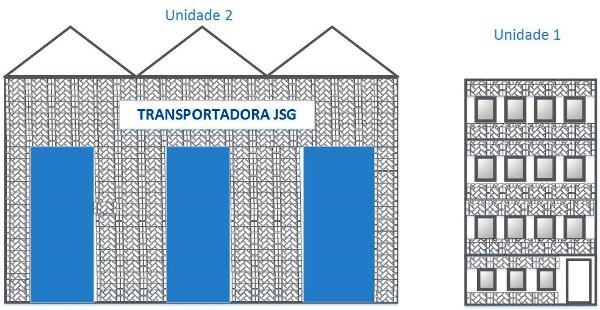
\includegraphics[]{fig1}
	\caption{Planta Física - Unidade 1 e 2}
	\label{fig1}
\end{figure}

\begin{figure}
	\centering
	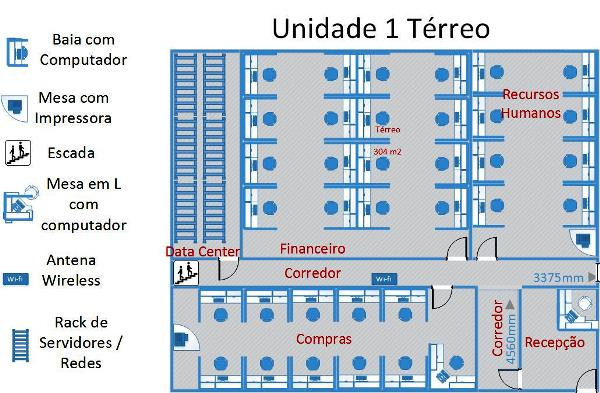
\includegraphics[]{fig2}
	\caption{Planta Física - Unidade 1 Térreo}
	\label{fig2}
\end{figure}

Departamento Financeiro

1 Rack com 2 Switch Cisco Catalyst 3560 48 Portas
2 Furukawa Patch Panel 48P 1U
DIO Distribuidor Interno Optico utilizado para interligar com o Switch Core do Data Center
16 pontos de Rede com uma distância média entre eles de 1,5 metros
Distância até o switch core no Data Center 30 metros
Horário de trabalho para implantação da rede após as 18:00

	
	 Departamento Recursos Humanos

Os pontos de rede é originado do rack do Departamento Financeiro
9 pontos de Rede com uma distância média entre eles de 1,5 metros
Uma distância média de 30 metros até o rack
Horário de trabalho para implantação da rede após as 18:00

	 Departamento Compras

1 Rack com 2 Switch Cisco Catalyst 3560 48 Portas
2 Furukawa Patch Panel 48P 1U
Distribuidor Interno Optico utilizado para interligar com o Switch Core do Data Center
12 pontos de Rede com uma distância média entre eles de 1,5 metros
Distância até o switch core no Data Center 50 metros
Horário de trabalho para implantação da rede após as 18:00


	 Departamento Recepção

Os pontos de rede é originado do rack do Departamento Financeiro
2 pontos de Rede com uma distância média entre eles de 1,5 metros
Uma distância média de 15 metros até o rack
Horário de trabalho para implantação da rede após as 18:00

	 Departamento Data Center

Onde se encontra o Switch Core da empresa que conecta todos os demais switchs dos setores através de fibra óptica
Rack com roteador, Cisco ASA, 2 Switch Cisco Catalyst 3560
8 Furukawa Patch Panel 48P 1U
Capacidade de 120 pontos de rede
Capacidade de 120 fibras(DIOS)
Uma distância média de 3 metros entre os racks de servidores
Horário de trabalho para implantação da rede após as 18:00
\\
\\
\\
\\
\\
\\
\\
\\
\\
\\
\\
\\
\\
\\
\\
\\
\\
\\
\\
\\
\\
\begin{figure}
	\centering
	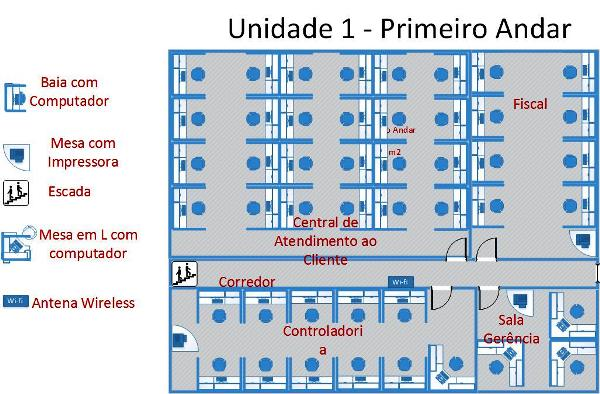
\includegraphics[]{fig3}
	\caption{Planta Física - Unidade 1 Primeiro Andar}
	\label{fig3}
\end{figure}

Departamento Central de Atendimento ao Cliente

1 Rack com 2 Switch Cisco Catalyst 3560 48 Portas
2 Furukawa Patch Panel 48P 1U
DIO Distribuidor Interno Optico utilizado para interligar com o Switch Core do Data Center
24 pontos de Rede com uma distância média entre eles de 1,5 metros
Distância até o switch core no Data Center 60 metros
Horário de trabalho para implantação da rede após as 18:00

	Departamento Fiscal

Os pontos de rede é originado do rack do Atendimento ao Cliente
9 pontos de Rede com uma distância média entre eles de 1,5 metros
Uma distância média de 15 metros até o rack
Horário de trabalho para implantação da rede após as 18:00

Departamento Controladoria

1 Rack com 2 Switch Cisco Catalyst 3560 48 Portas
2 Furukawa Patch Panel 48P 1U
DIO Distribuidor Interno Optico utilizado para interligar com o Switch Core do Data Center
12 pontos de Rede com uma distância média entre eles de 1,5 metros
Distância até o switch core no Data Center 80 metros
Horário de trabalho para implantação da rede após as 18:00

	Departamento Sala Gerência

Os pontos de rede é originado do rack da Controladoria
4 pontos de Rede com uma distância média entre eles de 1,5 metros
Uma distância média de 15 metros até o rack
Horário de trabalho para implantação da rede após as 18:00
\\
\\
\\
\\
\\
\\
\\
\\
\\
\\
\\
\begin{figure}
	\centering
	\includegraphics[]{fig4}
	\caption{Planta Física - Unidade 1 Segundo Andar}
	\label{fig4}
\end{figure}
Departamento Monitoramento

1 Rack com 2 Switch Cisco Catalyst 3560 48 Portas
2 Furukawa Patch Panel 48P 1U
DIO Distribuidor Interno Optico utilizado para interligar com o Switch Core do Data Center
40 pontos de Rede com uma distância média entre eles de 1,5 metros
Distância até o switch core no Data Center 100 metros
Horário de trabalho para implantação da rede após as 18:00

Departamento Comercial

1 Rack com 2 Switch Cisco Catalyst 3560 48 Portas 
2 Furukawa Patch Panel 48P 1U
DIO Distribuidor Interno Optico utilizado para interligar com o Switch Core do Data Center
12 pontos de Rede com uma distância média entre eles de 1,5 metros
Distância até o switch core no Data Center 100 metros
Horário de trabalho para implantação da rede após as 18:00

Departamento Sala Diretoria

Os pontos de rede é originado do rack da Comercial
4 pontos de Rede com uma distância média entre eles de 1,5 metros
Uma distância média de 15 metros até o rack
Horário de trabalho para implantação da rede após as 18:00
\\
\\
\\
\\
\begin{figure}
	\centering
	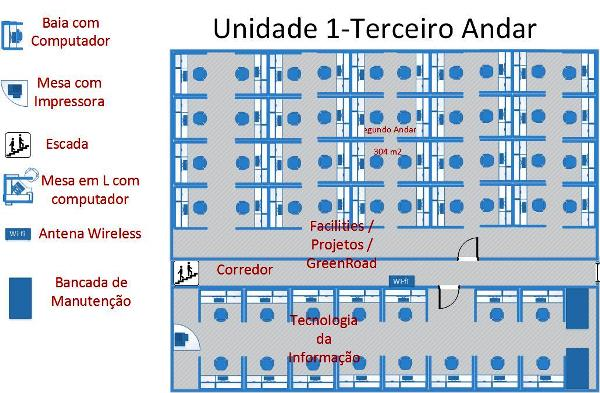
\includegraphics[]{fig5}
	\caption{Planta Física - Unidade 1 Terceiro Andar}
	\label{fig5}
\end{figure}

Departamento Facilities / Projetos / GreenRoad

1 Rack com 2 Switch Cisco Catalyst 3560 48 Portas
2 Furukawa Patch Panel 48P 1U
DIO Distribuidor Interno Optico utilizado para interligar com o Switch Core do Data Center
40 pontos de Rede com uma distância média entre eles de 1,5 metros
Distância até o switch core no Data Center 130 metros
Horário de trabalho para implantação da rede após as 18:00

	Departamento Tecnologia da Informação

1 Rack com 2 Switch Cisco Catalyst 3560 48 Portas
2 Furukawa Patch Panel 48P 1U
DIO Distribuidor Interno Optico utilizado para interligar com o Switch Core do Data Center
20 pontos de Rede com uma distância média entre eles de 1,5 metros
Distância até o switch core no Data Center 150 metros
Horário de trabalho para implantação da rede após as 18:00

	Departamento Tecnologia da Informação

1 Rack com 2 Switch Cisco Catalyst 3560 48 Portas
2 Furukawa Patch Panel 48P 1U
DIO Distribuidor Interno Optico utilizado para interligar com o Switch Core do Data Center
20 pontos de Rede com uma distância média entre eles de 1,5 metros
Distância até o switch core no Data Center 150 metros
Horário de trabalho para implantação da rede após as 18:00
\\
\\
\\
\\
\\
\\
\\
\\
\\
\\
\\
\\
\begin{figure}
	\centering
	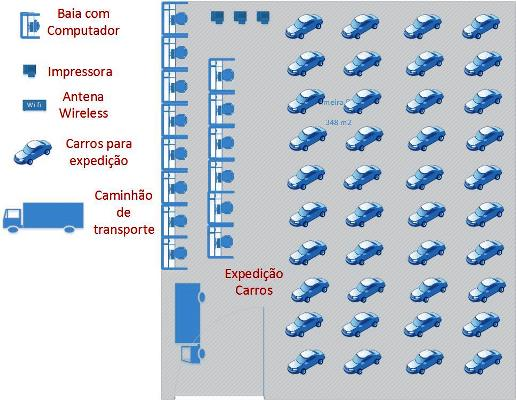
\includegraphics[]{fig6}
	\caption{Planta Física - Unidade 2 Doca 1 }
	\label{fig6}
\end{figure}
Rack com um Switch Core, roteador, Cisco ASA.
4 Furukawa Patch Panel 48P 1U
Rack com roteador, Cisco ASA, 2 Switch Cisco Catalyst 3560
16 pontos de Rede com uma distância média entre eles de 2,0 metros
Distância até o switch core no Data Center 20 metros
Horário de trabalho para implantação da rede após as 18:00
\\
\\
\\
\\
\\
\\
\\
\\
\\
\\
\\
\\
\\
\\
\\
\\
\\
\\
\\
\begin{figure}
	\centering
	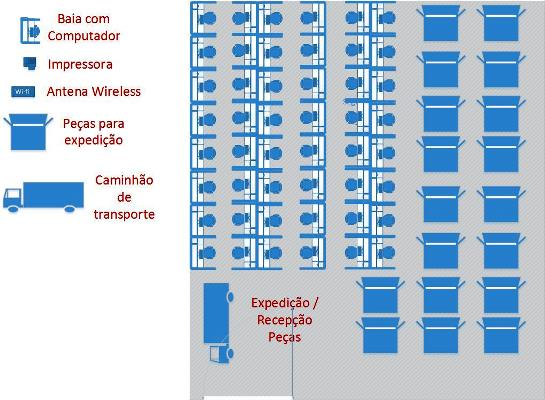
\includegraphics[]{fig7}
	\caption{Planta Física - Unidade 2 Doca 2 }
	\label{fig7}
\end{figure}

Rack com 2 Switch Cisco Catalyst 3560
2 Furukawa Patch Panel 48P 1U
48 pontos de Rede com uma distância média entre eles de 2,0 metros
Distância até o switch core no Data Center 100 metros
Horário de trabalho para implantação da rede após as 18:00
\\
\\
\\
\\
\\
\\
\\
\\
\\
\\
\\
\\
\\
\\
\\
\\
\\
\\
\\
\begin{figure}
	\centering
	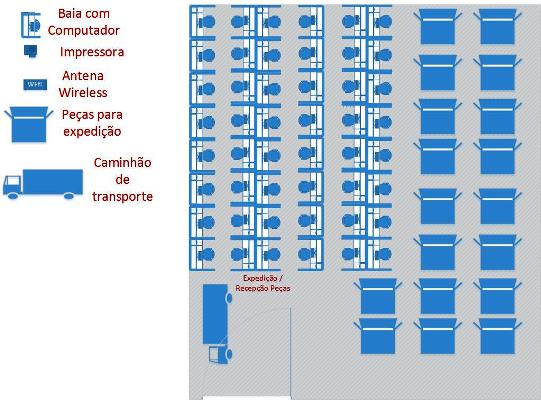
\includegraphics[]{fig8}
	\caption{Planta Física - Unidade 2 Doca 3 }
	\label{fig8}
\end{figure}
Rack com 2 Switch Cisco Catalyst 3560
2 Furukawa Patch Panel 48P 1U
48 pontos de Rede com uma distância média entre eles de 2,0 metros
Distância até o switch core no Data Center 250 metros
Horário de trabalho para implantação da rede após as 18:00

\subsection{Estado atual}
Abaixo será explicado a planta lógica e a topologia de rede adotada.


\subsection{Topologia}
Topologia das unidades 1 e 2 representadas na figura abaixo. Cada rack com o nome do setor terá 2 switchs de 48 portas “interligados” ao switch core através de fibra óptica, haverá um switch de 48 portas “nomeado” de switch de “acesso” no qual estará ligado o roteador e também o equipamento CiscoAsa que fará a VPN entre a unidade 1 e 2.
A unidade 1 terá 13 Switchs Cisco de 48 portas, 1 switch core 6509, 1 Cisco Asa e roteador.
A unidade 2 terá 7 Switchs Cisco de 48 portas, 1 switch core 6509, 1 Cisco ASA e roteador.

\begin{figure}
	\centering
	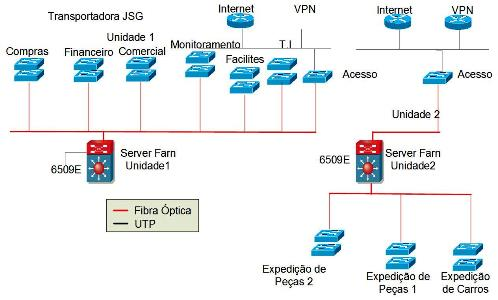
\includegraphics[]{fig9}
	\caption{Topologia }
	\label{fig9}
\end{figure} 
\begin{figure}
	\centering
	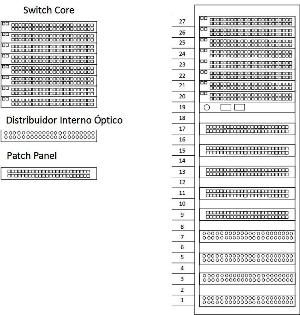
\includegraphics[]{fig10}
	\caption{O rack disponível no data center de cada unidade. }
	\label{fig10}
\end{figure} 
\begin{figure}
	\centering
	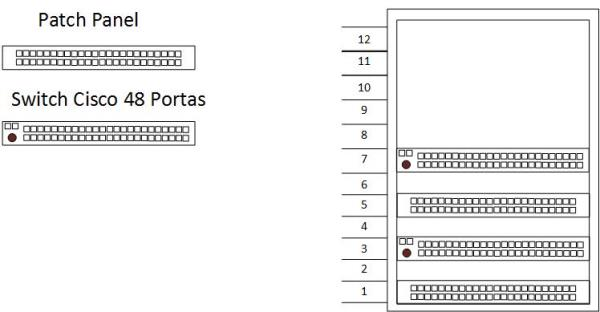
\includegraphics[]{fig11}
	\caption{O rack disponível nos setores. }
	\label{fig11}
\end{figure} 
\subsection{Encaminhamento}
Os cabos entre o switch localizado em cada setor e as estações de trabalho passaram por 2 canaletas de PVC de 60X50 mm de 2 metros fixada na parede, essa canaleta sairá do rack em direção as estações de trabalho.\\
Para interligação dos Switchs com o Switch Core no Data Center será utilizado Fibra Óptica, que passará dentro de uma Eletrocalha Perfurada de 50x100mm de três metros.
\\
\\
\\
\\
\\
\\
\\
\\
\\
\\
\\
\\
\\
\\
\\
\\
\\
\\
\\
\\
\\
\\
\\
\\
\\
\\
\\
\subsection{Memorial descritivo}

Abaixo a relação de todos os equipamentos passivos que serão utilizados no projeto:
\ref{tab7}.
\begin{table}[h!] % coloque h! para forcar a posicao
\centering
\caption{Memorial Descritivo}
\label{tab7} %com este label vc faz referencia no texto
\begin{tabular}{|l|l|l|l|}
\hline
Equipamento                    & Modelo        & Fabricante                & Quantidade \\ \hline
Patch Panel 48P 1U             & 35050805      & Furukawa                  & 36         \\ \hline
Canatela PVC 60X50 2 metros    & AC6050        & Helaclima HellermannTyton & 400        \\ \hline
Cabo de Rede CAT5E 25 Metros   & CAT5E         & Megatron                  & 24         \\ \hline
Eletrocalha 50x100 mm 3 metros & PL12          & Perfil Lider              & 380        \\ \hline
Fibra Óptica 2 Km              & ASU80M        & Fiber Home                & 1          \\ \hline
DIO 6 Portas                   & 35050381      & Furukawa                  & 14         \\ \hline
Cordão Óptico                  & 33000049      & Furukawa                  & 80         \\ \hline
Gbic                           & GLC-SX-MM-RGD & Cisco                     & 24         \\ \hline
RJ45 100PCS                    & RJ45-201      & Fortrek                   & 10         \\ \hline
Espelho 06 Posições            & 35050093      & Furukawa                  & 100        \\ \hline
Rotulador                      & PT-80         & Brother                   & 1          \\ \hline
\end{tabular}
\end{table}
\\
\\
\\
\\
\\
\\
\\
\\
\\
\\
\\
\\
\\
\\
\\
\\
\\
\\
\\
\\
\\

\subsection{Identificação dos cabos}
A identificação dos cabos de rede ocorrerá de acordo com o número do PatchPanel/Número da Porta do patch Panel.
Os Patchpanel serão numerados em sequencia(1,2,3 e etc) e os cabos de rede serão adesivados exemplo PP01-PT01 PP é o PatchPanel 1, PT é a porta onde será conectado, todos os patchs panel serão também eles identificados. A mesma regra será utilizada na fibra óptica e DIOS, conforme imagem abaixo:
\begin{figure}
	\centering
	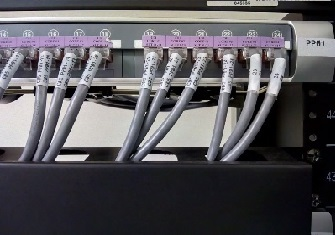
\includegraphics[]{fig12}
	\caption{Exemplo de identificação dos cabos}
	\label{fig12}
\end{figure} 


 \section{Implantação}
Hoje na empresa possuímos uma rede antiga ainda em operação, sendo substituído todos os equipamentos e infraestrutura antiga, a instalação dos equipamentos, infraestrutura, ocorrerá em paralelo com a existente hoje, após toda a instalação da nova infra e rede será removido e substituído a anterior.
O Horário de trabalho durante a semana será de 22:00 as 07:00, horário que não possui trabalho nos setores não gerando impactos desta forma, as atividades ocorrerão de segunda a sábado.
\\
\\
\\
\\
\\
\\
\\
\\
\\
\\
\\
\\
\\
\\
\\
\\
\\
\\
\\
\\
\\
\\
\\
\\
\\
\\
\\
\\
\\
\\
\\
\\
\\
\
 \begin{figure}
	\centering
	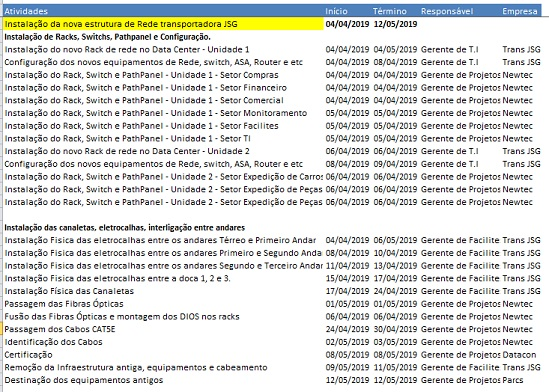
\includegraphics[]{fig13}
	\caption{Cronograma Implantação}
	\label{fig13}
\end{figure} 



\section{Plano de certificação}
A certificação da rede do projeto ocorrerá com a empresa DataCen que fará essa atividade, o primeiro passo para essa certificação é avaliar as condições da rede, infraestrutura, cabeamento e etc. Com a rede “em funcionamento” será realizado a certificação.\\ 
A certificação ocorrerá no dia 08/05/2019 com a rede em pleno funcionamento, será testado todos os pontos de rede e patch panel. 
Os relatórios de certificação que a empresa DataCen precisa entregar são TIA/EIA, TIA/EIA-568-B.2. 


\section{Plano de manutenção}

Toda a manutenção na rede será feita em conjunto com o time de Facilites e T.I, em um cronograma estabelecido, as manutenções ocorrerá a cada 3 meses, onde será feito a vistoria em toda a infraestrutura física. \\
A emissão de certificados de novos pontos será de responsabilidade da empresa Datatecn em um contrato anual estabelecido.

\subsection{Plano de expansão}
Todo o rack de setor possui um DIO com 4 pontos sobressalente para adição de novos switchs, além disso toda a infraestrutura foi dimensionada para suportar a passagem de mais cabos, suportando assim uma grande expansão caso seja necessária no futuro.

\section{Risco}
Toda as vezes que é realizado uma manutenção, criação ou alteração em uma rede ocorre risco para a organização que contratou ou está executando o serviço, os riscos identificados neste projeto foram:
Rede com oscilação enquanto é construída nova infraestrutura
Problemas de conectividade
Rede Wifi poderá haver quedas
Ponto de rede que possa não ter sido mapeado no projeto, o que demandará uma nova atividade local.

\section{Orçamento}
\ref{tab8}.
\begin{table}[h!] % coloque h! para forcar a posicao
\centering
\caption{Orçamento}
\label{tab8} %com este label vc faz referencia no texto
\begin{tabular}{|l|l|l|}
\hline
Equipamento                             & Fabricante                & Valor Total  \\ \hline
Patch Panel 48P 1U                      & Furukawa                  & 17.940,24    \\ \hline
Canatela PVC 60X50 2 metros             & Helaclima HellermannTyton & 20.360,00    \\ \hline
Cabo de Rede CAT5E 25 Metros            & Megatron                  & 2.253,60     \\ \hline
Eletrocalha 50x100 mm 3 metros          & Perfil Lider              & 18.202,00    \\ \hline
Fibra Óptica 2 Km                       & Fiber Home                & 4.581,99     \\ \hline
DIO 6 Portas                            & Furukawa                  & 2.099,72     \\ \hline
Cordão Óptico                           & Furukawa                  & 7.385,60     \\ \hline
Gbic                                    & Cisco                     & 48.621,36    \\ \hline
RJ45 100PCS                             & Fortrek                   & 327,20       \\ \hline
Espelho 04 Posições                     & Furukawa                  & 1.665,00     \\ \hline
Rotulador                               & Brother                   & 198,27       \\ \hline
Switch Core                             & Cisco                     & 160.000,00   \\ \hline
Switch 48 portas                        & Cisco                     & 953.902,60   \\ \hline
Asa                                     & Cisco                     & 4.000,00     \\ \hline
Serviço - Cerrtificação da rede         & 1                         & 30000,00     \\ \hline
Serviço - Configuração de rede          & 1                         & 35000,00     \\ \hline
Serviço - Infraestrutura Física         & 1                         & 50000,00     \\ \hline
Serviço - Instalação e estrutura Física & 1                         & 80000,00     \\ \hline
Total                                   & 1.436.537,58              & 1.436.537,58 \\ \hline
\end{tabular}
\end{table}
\section{Recomendações}
Após a entrega da rede pronta, é necessário que a empresa sempre atualize a documentação quando houver alterações na rede, é importante que toda modificação seja realizada por profissionais ou empresa especializada.
Toda a rede é composta de equipamento gerenciado, o que vai permitir maior segurança para a rede a partir do novo projeto.
\section{Referências bibliográficas}
TANENBAUM, Andrew S. Redes de Computadores. Rio de Janeiro, RJ: Editora
Campus – 3ª edição, 1997.
AWBES. Cabeamento Estruturado. Referência extraída da apostila Cabling I - Impacta
Tecnologia 
NETO, Vicente Soares, SILVA, Adelson de Paula, JÚNIOR, Mário Boscato C. Redes de
Alta Velocidade – Cabeamento Estruturado. São Paulo, SP: Editora Érica – 3ª edição,
2002.

\renewcommand\refname{} %%Referências bibliográficas}  
\bibliographystyle{ieeetr}
\bibliography{referencias}  



%% ***********************************************************************
%% === ate aqui    =====  ================================================
%% ***********************************************************************

\end{document}